\documentclass[10pt,fleqn]{article}
\usepackage{hyperref}
\usepackage{graphicx}


\setlength{\topmargin}{-.75in}
\addtolength{\textheight}{2.00in}
\setlength{\oddsidemargin}{.00in}
\addtolength{\textwidth}{.75in}

\nofiles

\pagestyle{empty}

\setlength{\parindent}{0in}

% new math commands


\setlength{\oddsidemargin}{-0.25in}
\setlength{\evensidemargin}{-0.25in}
\setlength{\textwidth}{6.75in}
\setlength{\headheight}{0.0in}
\setlength{\topmargin}{-0.25in}
\setlength{\textheight}{9.00in}

\makeindex

\usepackage{mathrsfs}

%\usepackage[pdftex]{graphicx}
\usepackage{epstopdf}

\newcounter{beans}

\newcommand{\ds}{\displaystyle}
\newcommand{\limit}[2]{\displaystyle\lim_{#1\to#2}}

\newcommand{\binomial}[2]{\ \left( \begin{array}{c}
                                  #1 \\
                                  #2
                                 \end{array}
                            \right) \
                         }
\newcommand{\ExampleRule}[2]
  {
  \noindent
  \rule{\linewidth}{1pt}
  \begin{example}
    #1
    \label{#2}
  \end{example}
  \rule{\linewidth}{1pt}
  \vskip0.125in
  }

\newcommand{\defbox}[1]
  {
   \ \\
   \noindent
   \setlength\fboxrule{1pt}
   \fbox{
        \begin{minipage}{6.5in}
          #1
        \end{minipage}
        }
   \ \\
  }
\newcommand{\verysmallworkbox}[1]
  {
   \ \\
   \noindent
   \setlength\fboxrule{1pt}
   \fbox{
        \begin{minipage}{6.5in}
           #1
           \ \\
           \vskip0.5in \ \\
           \ \\
        \end{minipage}
        }
   \ \\
  }
\newcommand{\smallworkbox}[1]
  {
   \ \\
   \noindent
   \setlength\fboxrule{1pt}
   \fbox{
        \begin{minipage}{6.5in}
           #1
           \ \\
           \vskip2.5in \ \\
           \ \\
        \end{minipage}
        }
   \ \\
  }
\newcommand{\halfworkbox}[1]
  {
   \ \\
   \noindent
   \setlength\fboxrule{1pt}
   \fbox{
        \begin{minipage}{6.5in}
           #1 \hfill
           \ \\
           \vskip3.25in \ \\
           \ \\
        \end{minipage}
        }
   \ \\
  }
\newcommand{\largeworkbox}[1]
  {
   \ \\
   \noindent
   \setlength\fboxrule{1pt}
   \fbox{
        \begin{minipage}{6.5in}
           #1
           \ \\
           \vskip7.5in \ \\
           \ \\
        \end{minipage}
        }
   \ \\
  }
\newcommand{\flexworkbox}[2]
  {
   \ \\
   \noindent
   \setlength\fboxrule{1pt}
   \fbox{
        \begin{minipage}{6.5in}
           #1
           \ \\

           \vskip#2 \ \\
           \ \\
        \end{minipage}
        }
   \ \\
  }


% symbols for sets of numbers

\newcommand{\natnumb}{$\cal N$}
\newcommand{\whonumb}{$\cal W$}
\newcommand{\intnumb}{$\cal Z$}
\newcommand{\ratnumb}{$\cal Q$}
\newcommand{\irrnumb}{$\cal I$}
\newcommand{\realnumb}{$\cal R$}
\newcommand{\cmplxnumb}{$\cal C$}

% misc. commands

\newcommand{\mma}{{\it Mathematica}}
\newcommand{\sech}{\mbox{ sech}}
 
\newtheorem{theorem}{Theorem}
\newtheorem{example}{Example}
\newtheorem{definition}{Definition}
\newtheorem{problem}{Problem}

\setcounter{secnumdepth}{2}
\setcounter{tocdepth}{4}


\begin{document}
%%%%%%%%%%%%%%%%%%%%%%%%%%%%%%%%%%%%%%%%%%%%%%%%%%%%%%%%%%%%%%%%%%%%%%%%%%%%%%%%
%%%%%%%%%%%%%%%%%%%%%%%%%%%%%%%%%%%%%%%%%%%%%%%%%%%%%%%%%%%%%%%%%%%%%%%%%%%%%%%%
\vskip0.1in\hrule\vskip0.1in
\noindent
{\bf Math 4610 Fundamentals of Computational Mathematics  - Topic 5.}
\vskip0.1in\hrule\vskip0.1in

This topic covers information on how to work once a terminal is up and running
on your computer. A Linux/Unix operating system should be running in the
terminal. In most real computational settings, it is important to be able to
work using a command line to create files, modify these files, compile
code, and a number of other tasks. You can invoke multiple terminals and work on
multiple files at the same time. Your instructor has three or four terminals
open at any given time. One to edit files, one to compile and execute code, and
the third to display results. The homework and projects assigned in the class
will typically require the use of a terminal to complete the work.

We will eventually use High Performance Computing (HPC) resources at the Center
for High Performance Computing (CHPC) at the University of Utah to work on a
project or two. The access these resources, we will need to do this through
terminals or terminal emulators running Linux/Unix operating systems. So, it is
important to be familiar with at least a few basic Linux/Unix commands. In this
section of the notes we will work through a few of the more important commands
needed. We will also introduce more commands with options as we work through the
semester.

In general, a Linux/Unix command can be written in the form:
\begin{verbatim}

    koebbe% command [options] [input parameters]

\end{verbatim}
where koebbe\% is the prompt for entering a command and \lq\lq command\rq\rq\ is
replaced with a command. For example, replacing \lq\lq command\rq\rq with
the string \lq\lq pwd\rq\rq gives
\begin{verbatim}

    koebbe% pwd 

\end{verbatim}
The options and parameters in the general form may or may not be needed
depending on what you are trying to do. Note that the pwd command will display
the (p)resent (w)orking (d)irectory. In most cases, the pwd command will not
need any options or parameters. When we compile code, it is common to use a
number of options on the compiler commands. For example, one of the assignments
will require the development of a shared library which entails compiling code in
multiple files and then archiving the compiled versions of the files into the
library - more on this later.

Each of the subsections below will cover a single type of command to help you
get started. There are hundreds of commands that can be used from within a
terminal. Some of these commands can be unforgiving - there is no trash folder
that will save you from accidently removing a file. Note that there are some
safety measures that one can add. See the file remove command (rm) below.

Another important issue that any computational person should be aware of is that
there are a number of shells that you can work in. A command shell, say bash,
will have a slightly different flavor of commands and syntax. The shells that
most computational scientists use are bash, csh, tcsh, and ksh. It is probably
best to select a shell, like bash or tcsh, and stick with that throughout the
semester. Finally, a good computational person is able to chain together a set
of commands to perform a sequence of commands. This sometimes referred to as
shell programming or shell scripting. This is an incredibly useful skill to
have. However, shell programming is beyond the scope of this course - meaning we
can get by without it.
%%%%%%%%%%%%%%%%%%%%%%%%%%%%%%%%%%%%%%%%%%%%%%%%%%%%%%%%%%%%%%%%%%%%%%%%%%%%%%%%
%%%%%%%%%%%%%%%%%%%%%%%%%%%%%%%%%%%%%%%%%%%%%%%%%%%%%%%%%%%%%%%%%%%%%%%%%%%%%%%%
\vskip0.1in\hrule\vskip0.1in
\noindent
{\large{\bf List the Contents of the Home Folder} }
\vskip0.1in\hrule\vskip0.1in
\noindent
Once a terminal is running, the first thing we probably want to do is to look at
what is in a the directory we are in. It is also important to know where you are
in a directory tree and the like. This also serves as a first linux or unix
command. In the screenshot below there are a couple of versions of a command
that will list files and folders with more or less information. Note that most
linux commands look like the general command form given above. The example in
the figure shows to versions of the \lq\lq ls\rq\rq\ command. The first is a
simple version that lists files in the folder. The second example adds the
\lq\lq\ -a\rq\rq\ flag. This results in a list of all files including hidden
files in the folder. The output shows a couple more files. The last example
uses the flag(s) \lq\lq\ -al\rq\rq\ which gives a long listing for the files in
the folder. There are lots of variations that can be used to obtain information
about the files in a folder.
\vskip0.1in\hrule\vskip0.1in
\vfill
\begin{figure}[h]
\centering
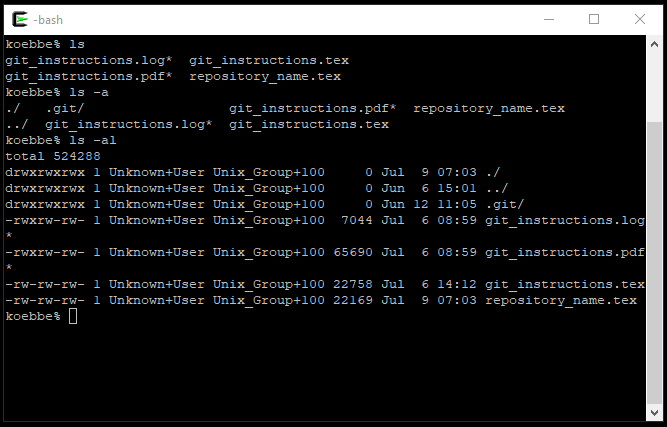
\includegraphics{../images/cygwin_02.png}
\caption{Three versions of the ls command used to list the contents of the
         curtent directory. Screenshot taken using {\bf Snip \& Sketch}. This is
         an app on my Windows 10 box}
\end{figure}
\eject
%%%%%%%%%%%%%%%%%%%%%%%%%%%%%%%%%%%%%%%%%%%%%%%%%%%%%%%%%%%%%%%%%%%%%%%%%%%%%%%%
%%%%%%%%%%%%%%%%%%%%%%%%%%%%%%%%%%%%%%%%%%%%%%%%%%%%%%%%%%%%%%%%%%%%%%%%%%%%%%%%
\vskip0.1in\hrule\vskip0.1in
\noindent
{\large{\bf Directory/Folder Commands}} 
\vskip0.1in\hrule\vskip0.1in
\noindent
You will need to create files and folders, move files and folders, remove files,
and perform other operations to directories to keep work organized. The
{\bf mkdir} command allows a persion to create a new directory in the current
working directory. This is the same thing tha Windows Explorer allows you to do
with a popup menu (New Folder). There will be many places where a directory
structure will be required. You can remove a directory with the {\bf rmdir}
command. The {\bf cd} command can be used to navigate through a directory
structure. Finally, on this screen capture, the {\bf pwd} command is used to
determine the current working directory. This can be used to figure out where
you are in a directory structure.
\begin{verbatim}

    koebbe% pwd                 current working directory
    koebbe% cd                  change working directory
    koebbe% mkdir               make a new directory
    koebbe% rmdir               remove an existing directory

\end{verbatim}
\vskip0.1in\hrule\vskip0.1in
\vfill
\begin{figure}[h]
\centering
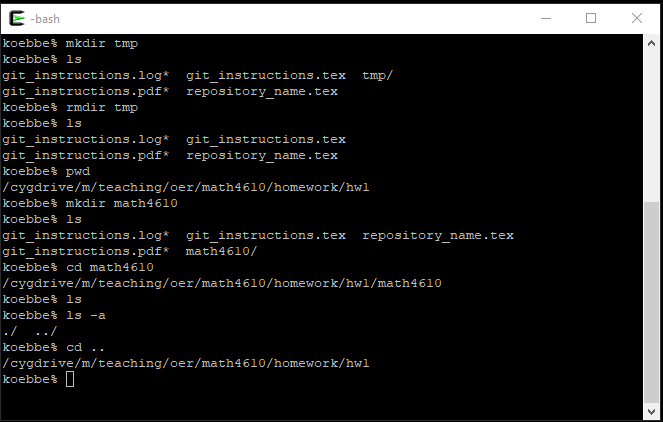
\includegraphics{../images/cygwin_03.png}
\caption{
  Commands for making and removing folders, changing the working directory and
  checking the location of the current folder files and folders. Screenshot
  taken using {\bf Snip \& Sketch}. This is an app on my Windows 10 box}
\end{figure}
\eject
\noindent
There are a few short cut commands for moving around your directory structure in
Linux. Here are a few that may save you some time.
\begin{verbatim}

    koebbe% cd ~                change working directory to the home directory
    koebbe% cd ..               change working directory to the parent directory
    koebbe% cd ../subfolder     change working directory up one folder and then
                                to subfolder 
    koebbe% cd subfolder        change working directory to a subfolder of the
                                current folder
    koebbe% cd ./subfolder      same as above
    koebbe% mkdirs folder       make the specfied folder and all subfolders
    koebbe% rmdir -rf folder    remove an existing directory with prejudice

\end{verbatim}
%%%%%%%%%%%%%%%%%%%%%%%%%%%%%%%%%%%%%%%%%%%%%%%%%%%%%%%%%%%%%%%%%%%%%%%%%%%%%%%%
%%%%%%%%%%%%%%%%%%%%%%%%%%%%%%%%%%%%%%%%%%%%%%%%%%%%%%%%%%%%%%%%%%%%%%%%%%%%%%%%
\vskip0.1in\hrule\vskip0.1in
\noindent
{\large{\bf The which and man Commands}} 
\vskip0.1in\hrule\vskip0.1in
\noindent
You will probably want to know what is available for doing work within Cygwin
or any other terminal emulator. The which command allows you determine if apps
or other executables are available on your version of Cygwin. In particular, it
is important to know if certain compilers (e.g, javac, gcc, f77) are available.
A significant number of tasks you will be asked to complete will require the use
of a compiler and Cygwin has a number of (good) standard compilers for C, C++,
and fortran. The syntax for the command is the following.
\begin{verbatim}

    koebbe% which command-name

\end{verbatim}
If the command results in command not found, this means that you typed the name
incorrectly (a constant source of frustration for your instructor) or the app
or command has not been installed. If in Cygwin, you can use the setup script to
find and install what is needed.

In the example shown below, the which command is used to test for 4 different
compilers. In each case, the location of the file associated with the command is
given. Once you know a command is available, you can use the man command to get
information about command usage. For example, typing
\begin{verbatim}

    koebbe% man gcc

\end{verbatim}
will display information on the gcc compiler along with explanations and
documentation on how to specify flags and options for the compiler.
\vskip0.1in\hrule\vskip0.1in
\vfill
\begin{figure}[h]
\centering
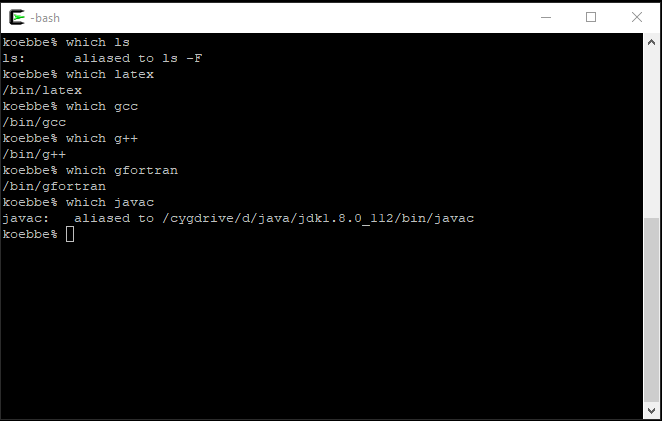
\includegraphics{../images/cygwin_04.png}
\caption{Using the which command to determine if compilers are installed.
         Screenshot taken using {\bf Snip \& Sketch}. This is an app on my
         Windows 10 box}
\end{figure}
\eject
%%%%%%%%%%%%%%%%%%%%%%%%%%%%%%%%%%%%%%%%%%%%%%%%%%%%%%%%%%%%%%%%%%%%%%%%%%%%%%%%
%%%%%%%%%%%%%%%%%%%%%%%%%%%%%%%%%%%%%%%%%%%%%%%%%%%%%%%%%%%%%%%%%%%%%%%%%%%%%%%%
\vskip0.1in\hrule\vskip0.1in
\noindent
{\large{\bf A Simple Editing Program}} 
\vskip0.1in\hrule\vskip0.1in
\noindent
You will need an editor to create text files. There are a number of editors that
can be downloaded and used in any Cygwin installation. The standard editor that
is always available for linux and unix boxes is \lq vi\rq\. This editor is a bit
rudimentary, but works. Another editor which will be used in by the instructor
in the course is \lq vim\rq, a modified and improved version of vi. The syntax
for starting the editor in a window is the following.
\begin{verbatim}

    koebbe% vim filename

\end{verbatim}
There are a lot of escape sequences vim uses to insert text, write a file and
so on. If you are new to vim, you will need to learn at least a few of these
editing commands.
\vskip0.1in\hrule\vskip0.1in
\vfill
\begin{figure}[h]
\centering
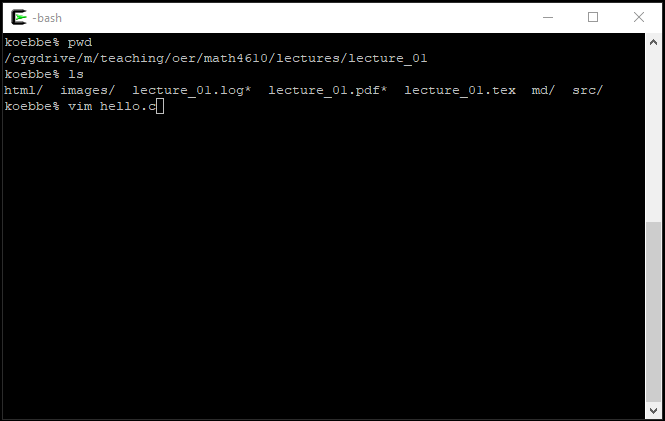
\includegraphics{../images/cygwin_05.png}
\caption{How to start the vim editor. Screenshot taken using vim. The name of 
         the file being edited is hello.c. {\bf Snip \& Sketch}. This is an app
         on my Windows 10 box}
\end{figure}
\eject
%%%%%%%%%%%%%%%%%%%%%%%%%%%%%%%%%%%%%%%%%%%%%%%%%%%%%%%%%%%%%%%%%%%%%%%%%%%%%%%%
%%%%%%%%%%%%%%%%%%%%%%%%%%%%%%%%%%%%%%%%%%%%%%%%%%%%%%%%%%%%%%%%%%%%%%%%%%%%%%%%
\vskip0.1in\hrule\vskip0.1in
\noindent
{\large{\bf First View of the vim Editor}} 
\vskip0.1in\hrule\vskip0.1in
\noindent
The terminal will turn what is shown below into when you start up the editor on
a new file. To get out of the editor, you can use any of the following commands
inside the editor.
\begin{verbatim}

    :x                  write and exit the editor - saves changes in the file
    :q                  exit the editor if no changes have been made
    :x!                 force a write and exit the editor - saves the file
    :q!                 force an exit of the editor - no changes are saved

\end{verbatim}
You need to type in the colon, :, to indicate you want to enter a command. Note
that there are a few other commands that can be used to save changes. For
example
\begin{verbatim}

    :w                  write and stay in the editor
    :w!                 force a write and stay in the editor

\end{verbatim}
\vskip0.1in\hrule\vskip0.1in
\vfill
\begin{figure}[h]
\centering
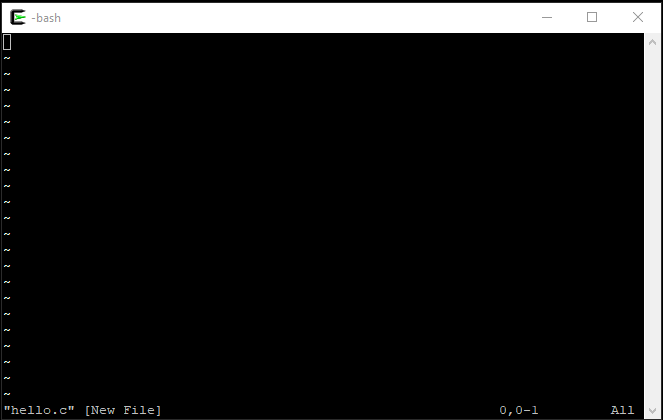
\includegraphics{../images/cygwin_06.png}
\caption{Opening up a new file in vim. Screenshot taken using
         {\bf Snip \& Sketch}. This is an app on my Windows 10 box}
\end{figure}
\eject
%%%%%%%%%%%%%%%%%%%%%%%%%%%%%%%%%%%%%%%%%%%%%%%%%%%%%%%%%%%%%%%%%%%%%%%%%%%%%%%%
%%%%%%%%%%%%%%%%%%%%%%%%%%%%%%%%%%%%%%%%%%%%%%%%%%%%%%%%%%%%%%%%%%%%%%%%%%%%%%%%
\vskip0.1in\hrule\vskip0.1in
\noindent
{\large{\bf An Example of a Text File/Program}}
\vskip0.1in\hrule\vskip0.1in
\noindent
The following screenshot shows a few lines that have been typed into vim that
deinfes a standard hello world example for C. To insert/append characters in the
text file, you can use the following commands to do this. Note that the commands
below do not show up on the screen and the chnages are made where the cursor is
currently located.
\begin{verbatim}

    a                     append text at this point in the file
    o                     open a line after the current line
    O                     open a line before the current line

\end{verbatim}
To end adding or inserting text, use a single escape character. Again, the
commands will not show up on screen. Learning everything about vi or vim is a
time consuming process. It is one of those things that you figure out as you go.
The advantage of vi is that it exists on every flavor of Linux/Unix.
\vskip0.1in\hrule\vskip0.1in
\vfill
\begin{figure}[h]
\centering
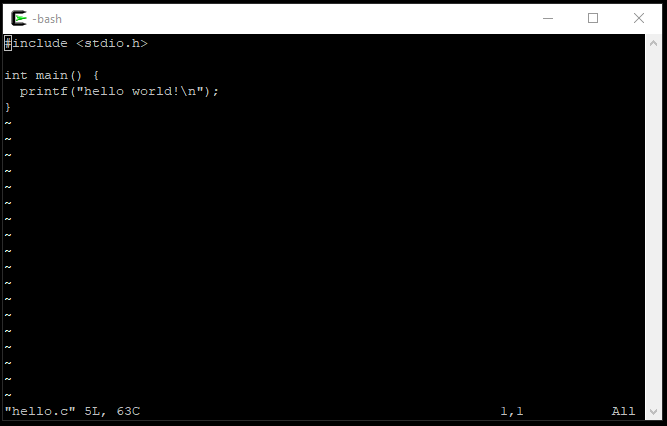
\includegraphics{../images/cygwin_07.png}
\caption{Adding lines to a text file. The text gives an example of the \lq\lq
         hello world\rq\rq\ program from a C course. Screenshot taken using
         {\bf Snip \& Sketch}. This is an app on my Windows 10 box}
\end{figure}
\eject
%%%%%%%%%%%%%%%%%%%%%%%%%%%%%%%%%%%%%%%%%%%%%%%%%%%%%%%%%%%%%%%%%%%%%%%%%%%%%%%%
%%%%%%%%%%%%%%%%%%%%%%%%%%%%%%%%%%%%%%%%%%%%%%%%%%%%%%%%%%%%%%%%%%%%%%%%%%%%%%%%
\vskip0.1in\hrule\vskip0.1in
\noindent
{\large{\bf Compiling a Program}}
\vskip0.1in\hrule\vskip0.1in
\noindent
Compiling a program is relatively easy at this point in time. To compile the
program shown in the previous section you can type:
\begin{verbatim}

    koebbe% gcc hello.c

\end{verbatim}
The result is an exeutable as seen below. If you want to name the executable
something besides \lq a\rq\ then type the following.
\begin{verbatim}

    koebbe% gcc -o hello hello.c

\end{verbatim}
\vskip0.1in\hrule\vskip0.1in
\vfill
\begin{figure}[h]
\centering
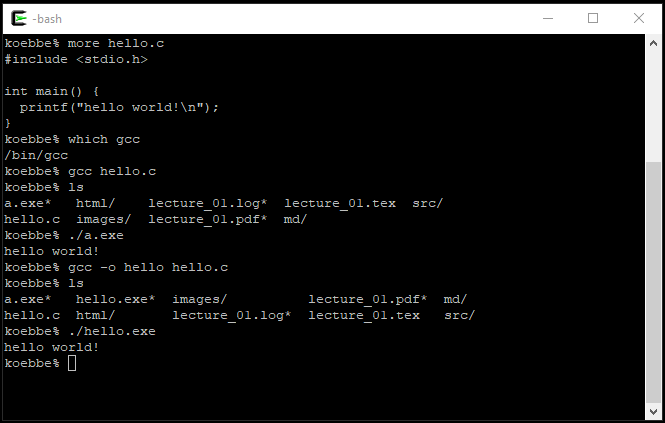
\includegraphics{../images/cygwin_08.png}
\caption{Compiling the hello.c program. Screenshot taken using
        {\bf Snip \& Sketch}. This is an app on my Windows 10 box}
\end{figure}
\eject
%%%%%%%%%%%%%%%%%%%%%%%%%%%%%%%%%%%%%%%%%%%%%%%%%%%%%%%%%%%%%%%%%%%%%%%%%%%%%%%%
%%%%%%%%%%%%%%%%%%%%%%%%%%%%%%%%%%%%%%%%%%%%%%%%%%%%%%%%%%%%%%%%%%%%%%%%%%%%%%%%
\vskip0.1in\hrule\vskip0.1in
\noindent
{\large{\bf Keeping Track of Working Code}}
\vskip0.1in\hrule\vskip0.1in
\noindent
It is a good idea to organize your work within assignments and projects. There
is a standard set of folders/directories in linux and unix that most have
adopted. Your instructor follows this idea and usually creates a list of
folders including /src, /data, /bin, and /doc. When computer literate folks see
these folders, they know what is stored in the folders. As an example, type the
commands
\begin{verbatim}

    koebbe% mkdir src
    koebbe% mkdir bin

\end{verbatim}
to create folders for the executable the text file: src for the text files and
bin for the binary/executable files. 
\vskip0.1in\hrule\vskip0.1in
\vfill
\begin{figure}[h]
\centering
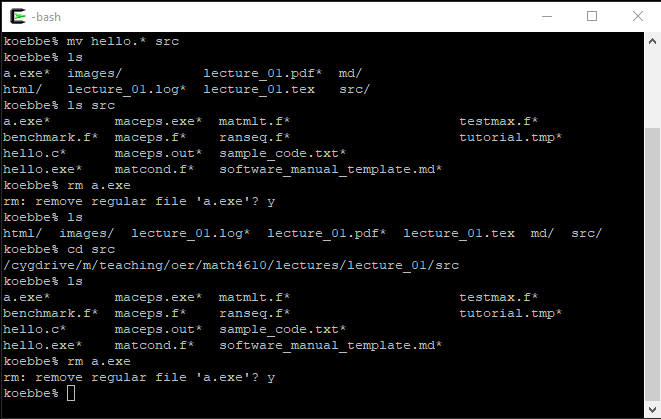
\includegraphics{../images/cygwin_09.png}
\caption{Some commands to reorganize files. Screenshot taken using
         {\bf Snip \& Sketch}. This is an app on my Windows 10 box}
\end{figure}
%%%%%%%%%%%%%%%%%%%%%%%%%%%%%%%%%%%%%%%%%%%%%%%%%%%%%%%%%%%%%%%%%%%%%%%%%%%%%%%%
%%%%%%%%%%%%%%%%%%%%%%%%%%%%%%%%%%%%%%%%%%%%%%%%%%%%%%%%%%%%%%%%%%%%%%%%%%%%%%%%
\vskip0.1in\hrule\vskip0.1in \noindent
  \href{../../topic_04/md/topic_04.md}{Previous} |
  \href{../../toc/md/topic_toc.md}{Table of Contents} |
  \href{../../topic_06/md/topic_06.md}{Next}
\vskip0.1in\hrule\vskip0.1in \noindent
%%%%%%%%%%%%%%%%%%%%%%%%%%%%%%%%%%%%%%%%%%%%%%%%%%%%%%%%%%%%%%%%%%%%%%%%%%%%%%%%
%%%%%%%%%%%%%%%%%%%%%%%%%%%%%%%%%%%%%%%%%%%%%%%%%%%%%%%%%%%%%%%%%%%%%%%%%%%%%%%%
\end{document}
